\section{Mehrgitterverfahren}

\textbf{Idee:} Ausnutzen mehrerer Diskretisierungslevel bei partiellen Differentialgleichungen.

\begin{bsp}[Mehrgitterverfahren f�r Modellproblem I]
Gegeben sei also $N,\ h:=\frac{1}{N+1}$ und der zugeh�rige 5-Punkte-Stern. Des Weiteren sei
\[
	\Omega_h:=\{(ih,jh):\ i,j=1,\ \ldots,\ N\}
\]
das zugeh�rige Gitter (ohne R�nder). Mit $A_h$ bezeichnen wir die zugeh�rige Laplace-Matrix
zur Diskretisierungsweite $h$.

\medskip

Bekannt ist:
\begin{lem} Die Matrix $A_h$ besitzt die Eigenwerte
\[
	\lambda_{k,l}:=4-2\left(\cos\left(\pi\cdot k\cdot h \right)+\cos\left(\pi\cdot l\cdot h \right) \right) \quad k,\ l=1,\  \ldots,\ N
\]
und die zugeh�rigen Eigenvektoren sind gegeben durch
\[
	z^{(k,l)}_{i,j}:=\sin(i\cdot k\cdot \pi\cdot h)\cdot\sin(j\cdot l\cdot \pi\cdot h) \quad k,\ l =1,\ \ldots,\ N.
\]
\end{lem}

\begin{aufg} \label{laplaceev_aufg}
Plotte $z^{(k,l)}$ f�r verschiedene Werte von $k,l$ mit Matlab (\texttt{mesh}), insbesondere f�r
\begin{enumerate}
\item $k=1,\ l=1$,
\item $k=2,\ l=1$,
\item $k=2,\ l=2$,
\item $k=\frac{N}{2},\ l=\frac{N}{2}$,
\item $k=N,\ l=N$,
\end{enumerate}
f�r $N\approx 32,\ 64$.
\end{aufg}

\begin{figure}
\centerline{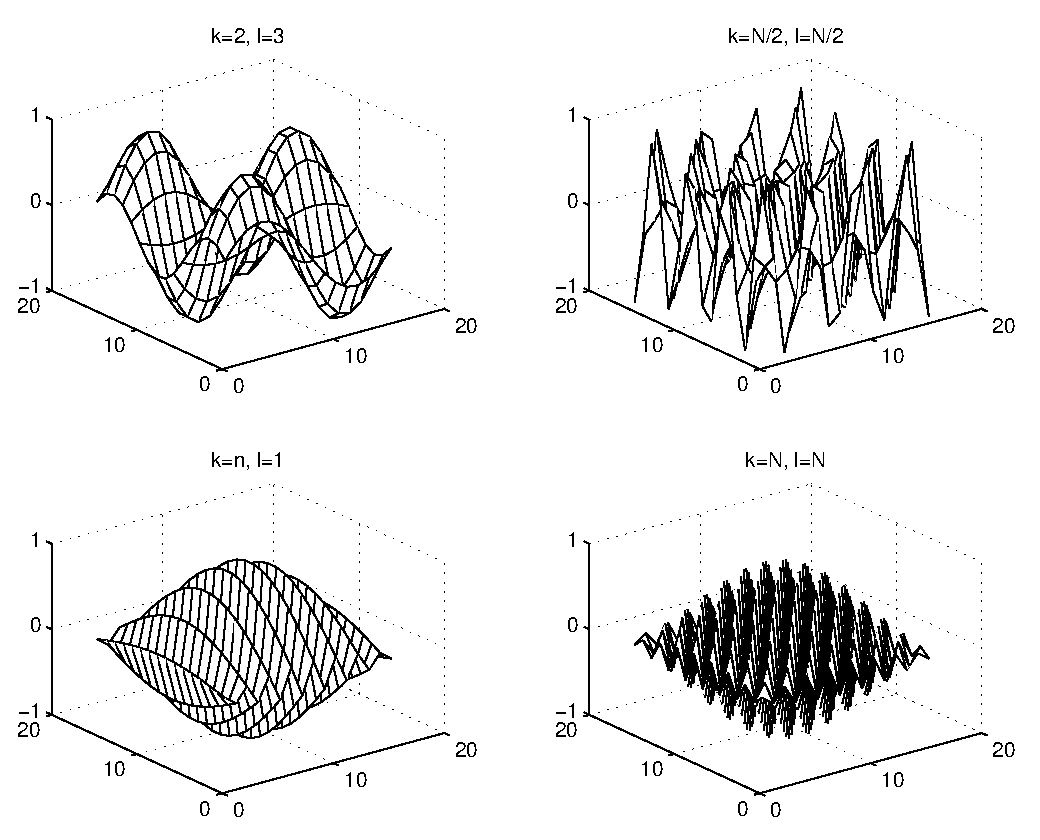
\includegraphics[scale=0.7]{eps/laplaceev}}
\caption{Ausgew\"ahlte Eigenvektoren f\"ur Modellproblem I}
\end{figure}

\subsection{Zweigitter-Verfahren}
Die Idee beim Zweigitter-Verfahren ist es jetzt, die L�sung f�r  $A_h$
durch eine L�sung f�r ein kleineres System
$A_{\hat h}$ mit gr\"o"serer Diskretisierungsweite $\hat{h}$ zu approximieren:
\begin{center}
\begin{picture}(125,85)
\drawline(0,80)(0,0)(120,0)(120,80)
\multiput(20,20)(40,0){3}{\circle{6}}
\multiput(40,20)(40,0){2}{\circle*{6}}
\multiput(20,40)(20,0){5}{\circle{6}}
\multiput(20,60)(40,0){3}{\circle{6}}
\multiput(40,60)(40,0){2}{\circle*{6}}
\end{picture}
\end{center}
Hier gilt $N=2\hat N+1$, also $\hat h=2\cdot h$.

\medskip

Wie Aufgabe~\ref{laplaceev_aufg} zeigt, gibt es Eigenvektoren, die einer starken Variation unterliegen, und Eigenvektoren, welche
eher "`glatt"' sind. Beim Verkleinern der Punktzahl jedoch k�nnen stark variierenden Eigenvektoren nur schlecht
approximiert werden. Darum unterteilen wir ($z^{(k,l)}$ seien Eigenvektoren f\"ur $A_h$)
\begin{align*}
X&:=\langle z^{(k,l)},\; k,\ l=1,\ \ldots,\ \hat N\rangle \quad (\text{"`glatte Vektoren"'} )\\
Y&:=\langle z^{(k,l)},\; k>\hat N \text{ oder } l>\hat N\rangle \quad (\text{"`oszillierende Vektoren"'} ).
\end{align*}

Es gilt dabei
\[
	\mathbb{R}^n=X\oplus Y \quad (n=N^2),
\]
weil die Eigenvektoren paarweise orthogonal zueinander sind.

\bigskip

Wir entwickeln nun ein Iterationsverfaren (�hnlich dem Schwarz-Verfahren) der folgenden Gestalt:

\fbox{\parbox{\linewidth-7pt}{
Gesucht ist der Fehler $e^k$ mit $x^*=x^k+e^k$. Statt dessen betrachten wir $r^k=b-A_h x^k$ (denn $A_he^k = A_h(x^*-x^k) = b - A_hx^k = r^k$).
\begin{enumerate}
\item Gl�tte $r^k$, d.h. bestimme $y^k$ so dass f\"ur $
s^k=b-A_hy^k$ gilt
\[
s^k \in X.
\]

\item Transportiere $s^k$ auf das grobe Gitter und bezeichne das Ergebnis mit $\hat s^k$. L�se
\[
A_{\hat h}\hat e^k=\hat s^k.
\]
Transportiere $\hat e^k$ auf das feine Gitter in $e^k$ und setze
\[
x^{k+1}=y^k+e^k.
\]
\end{enumerate}
}}

Anschaulichen entfernen wir aus $r^k$ die stark oszillierenden Komponenten.
\end{bsp}

\begin{defn}[Transportoperationen]
\begin{enumerate}
\item Die {\em Prolongation} $P$ (Abbildung von $\Omega_{\hat h}$ nach $\Omega_h$) ist als gewichtete Mittelung der acht Nachbar-Werte
definiert.
\begin{center}
\begin{picture}(190,160)
\multiput(20,0)(40,0){5}{\circle{6}}
\multiput(20,40)(80,0){3}{\circle{6}}
\multiput(60,40)(80,0){2}{\circle*{6}}
\multiput(20,80)(40,0){5}{\circle{6}}
\multiput(20,120)(80,0){3}{\circle{6}}
\multiput(60,120)(80,0){2}{\circle*{6}}
\multiput(20,160)(40,0){5}{\circle{6}}
\put(60,40){\vector(1,1){38}}
\put(140,40){\vector(-1,1){38}}
\put(60,120){\vector(1,-1){38}}
\put(140,120){\vector(-1,-1){38}}

\put(60,40){\vector(1,0){36}}
\put(140,40){\vector(-1,0){36}}

\put(75,110){$\frac{1}{4}$}
\put(120,110){$\frac{1}{4}$}

\put(59,50){$\frac{1}{4}$}
\put(135,50){$\frac{1}{4}$}

\put(80,25){$\frac{1}{2}$}
\put(115,25){$\frac{1}{2}$}
\end{picture}
\end{center}
bzw. in Sternform
\[
P=\left]\begin{array}{ccc}
\frac{1}{4}&\frac{1}{2}&\frac{1}{4}\\
\frac{1}{2}&1&\frac{1}{2}\\
\frac{1}{4}&\frac{1}{2}&\frac{1}{4}
\end{array}\right[ \quad  .
\]
$P$ ist eine $(\hat n\times n)$-Matrix, in welcher der Stern �ber die Zeilen verteilt ist. Dies ist eine bilineare Interpolation.

\item Die {\em Restriktion} $R$ als Abbildung von $\Omega_{ h}$
nach $\Omega_{\hat h}$ ist gegeben durch
\begin{center}
\begin{picture}(110,110)
\multiput(20,20)(40,0){3}{\circle{6}}
\multiput(20,60)(80,0){2}{\circle{6}}
\multiput(60,60)(80,0){1}{\circle*{6}}
\multiput(20,100)(40,0){3}{\circle{6}}

\put(20,20){\vector(1,1){38}}
\put(100,20){\vector(-1,1){38}}
\put(20,100){\vector(1,-1){38}}
\put(100,100){\vector(-1,-1){38}}

\put(20,60){\vector(1,0){36}}
\put(100,60){\vector(-1,0){36}}
\put(60,20){\vector(0,1){36}}
\put(60,100){\vector(0,-1){36}}

\put(8,97){$\frac{1}{16}$}
\put(8,57){$\frac{1}{8}$}
\put(8,17){$\frac{1}{16}$}

\put(105,97){$\frac{1}{16}$}
\put(105,57){$\frac{1}{8}$}
\put(105,17){$\frac{1}{16}$}

\put(65,97){$\frac{1}{8}$}
\put(65,17){$\frac{1}{8}$}
\put(70,60){$\frac{1}{4}$}
\end{picture}
\end{center}
bzw. in Sternform
\[
R=\frac{1}{4} \cdot \left]\begin{array}{ccc}
\frac{1}{4}&\frac{1}{2}&\frac{1}{4}\\
\frac{1}{2}&1&\frac{1}{2}\\
\frac{1}{4}&\frac{1}{2}&\frac{1}{4}
\end{array}\right[ \quad  .
\]
\end{enumerate}
Es gilt also $R=\frac{1}{4}\cdot P^T, \quad R\in\mathbb{R}^{\hat n \times n}, \quad P\in\mathbb{R}^{n \times \hat n},\ n=N^2,\ \hat n =\hat N^2$.
\end{defn}

\begin{bem}Die triviale Restriktion 
\[
R=
\left]\begin{array}{ccc}
0&0&0\\
0&1&0\\
0&0&0
\end{array}\right[
\]
ist f�r die Theorie und die Praxis weniger geeignet.
\end{bem}

Um die Frage des "`Gl�ttens"' zu behandeln, betrachten wir  das ged�mpfte Gesamschritt-Verfahren
\[
	y^{\nu+1}=y^\nu+\omega\cdot  D^{-1} r^\nu, \quad \omega \text{ D�mpfungsfaktor,}
\]
wobei $A=D-B,\ D=\diag(A),\ \nu=0,\ 1,\ \ldots$ Es gilt
\[
	r^{\nu+1}=((1-\omega ) I+\omega D^{-1}B)r^\nu.
\]
Setze $J_\omega:=(1-\omega ) I+\omega D^{-1}B$. Wir wissen: $J_\omega$ besitzt die Eigenvektoren $z^{(k,l)}$ mit den Eigenwerten
\[
	\mu_{k,l}^{(\omega)}=\frac{\omega}{2}\left(\cos(\pi\cdot k\cdot h)+\cos(\pi\cdot l\cdot h) \right)+(1-\omega).
\]
F�r die oszillierenden Eigenvektoren (d.h. $k>\frac{N-1}{2}$ oder $l>\frac{N-1}{2}$) gilt:
\[
	-2<\cos(\pi\cdot k\cdot h)+\cos(\pi\cdot l\cdot h)<1,
\]
also gilt f\"ur diese $k$ und $l$
\[
	|\mu_{k,l}^{(\omega)}|\le \max\left\{ \left|1-\frac{\omega}{2}\right|,\ |1-2\omega|\right \}, \quad  \omega>0.
\]
Die rechte Seite wird minimal f�r $\omega=\frac{4}{5}$ mit Wert $\frac{3}{5}$. 

\medskip

Wir halten fest:
\begin{lem} F�r $\omega\in\left[0,\frac{4}{5} \right]$ gilt
\begin{align*}
\frac{\omega}{2}\left(\cos(\pi\cdot k\cdot h)+\cos(\pi\cdot l\cdot h) \right)+(1-\omega)
	&\le  \max\left\{ \left|1-\frac{\omega}{2}\right|,\ |1-2\omega|\right \}\\
	&=1-\frac{\omega}{2}.
\end{align*}
\end{lem}

Damit haben wir alle Zutaten f�r ein Zweigitter-Verfahren beisammen.

\begin{defn} $y=S_{\nu,\omega}(x)$ bedeute $\nu$ Schritte der Gl�tterungsiteration angewendet auf $x$.
\end{defn}

\begin{alg}[Zweigitter-Verfahren]
~               % um "Algorithmus" aus dem Kasten rauszubekommen
\vspace*{-2\baselineskip}       % um den Leeraum zu entfernen
\begin{algorithm}
\begin{algorithmic}
\STATE w�hle $x^0$, setze $r^0=b-A_h x^0,\ \omega=\frac{4}{5}$
\FOR{$k=0,\ 1,\ \ldots$}
\STATE $y^k = S_{\nu,\omega}(x^k)$
\STATE $s^k = b-A_hy^k$ \COMMENT{$s^k$ ist glatt}
\STATE $\hat s^k = Rs^k$
\STATE l�se $A_{\hat h}\hat e^k = \hat s^k$
\STATE $e^k = P\hat e^k$
\STATE $x^{k+1} = x^k+e^k$
\ENDFOR
\end{algorithmic}
\end{algorithm}
\end{alg}

\begin{aufg}
Implementiere das Zweigitter-Verfahren f�r das Modellproblem I. Verwende direkten L�ser f�r $A_{\hat h}$ und messe
die Iterationszahlen abh�ngig von $\nu$ und $h$.
\end{aufg}

\begin{figure}[h!]
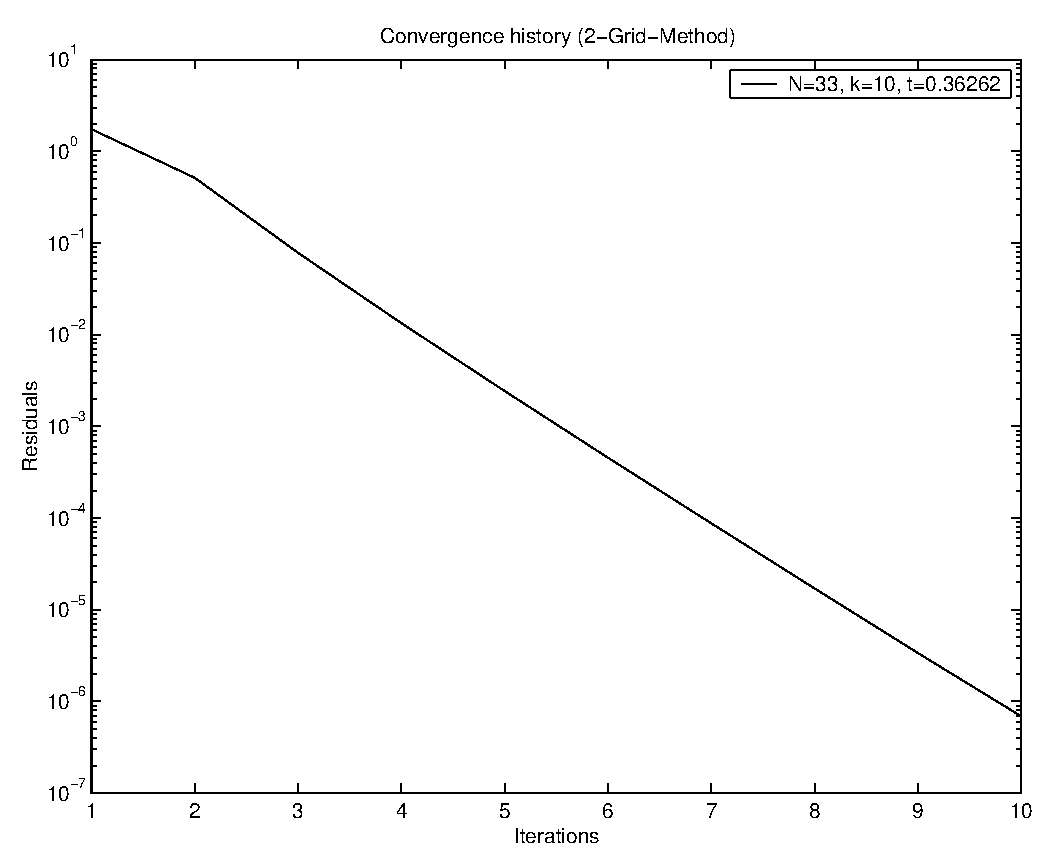
\includegraphics[scale=0.37]{eps/mp1mg2N33.eps}\hfill
\includegraphics[scale=0.37]{eps/mp1mg2N65.eps}
\caption{Zweigitterverfahrten f\"ur Modellproblem 1, $N=33$ (links), $N=65$ (rechts)}
\end{figure}

\subsection{Mehrgitter-Verfahren}
Die L�sung von $A_{\hat h}\hat e^k=\hat s^k$ kann auch rekursiv erfolgen. Man hat dann eine Hierachie: \\
$A_{0}$: zu l�sendes System \\
$A_{1}$: kleineres System mit zugeh�rigen Operatoren $P_1$ und $R_1$
\begin{center}
 $\vdots$
\end{center}
$A_{l_{max}}$: kleinstes System mit Operatoren $P_{l_{max}}$ und $R_{l_{max}}$ \\

Dem entspricht eine Hierachie von Gl�ttern: \\
$S^0_{\nu, \omega}$\\
\hspace*{0.25cm}$\vdots$ \\
$S^{l_{max}}_{\nu, \omega}$ \\

Das Mehrgitter-Verfahren ist dann gegeben durch:
\begin{alg}[Mehrgitter-Verfahren]
~               % um "Algorithmus" aus dem Kasten rauszubekommen
\vspace*{-2\baselineskip}       % um den Leeraum zu entfernen
\begin{algorithm}
\begin{algorithmic}
\STATE w�hle $x^0$, w"ahle $\gamma \in \{1,2,\ldots\}$ 
\FOR{$k=0,\ 1,\ \ldots$}
\item  $x^{k+1} = mgs(x^k, b, \gamma , 0 )$ \\
\ENDFOR
\end{algorithmic}
\end{algorithm}
\end{alg}

\begin{bem}
Dabei ist $mgs$ der noch zu definierende Mehrgitter-Schritt.
\end{bem}

\begin{alg}[Mehrgitter-Schritt $y = mgs(x, r,\gamma,l)$]
~               % um "Algorithmus" aus dem Kasten rauszubekommen
\vspace*{-2\baselineskip}       % um den Leeraum zu entfernen
\begin{algorithm}
\begin{algorithmic}[1]
%\IF{ $l=l_{max}$}
%\STATE l�se $A_{l_{max}} y = r$
%\ELSE
\STATE $x = S^l_{\nu, \omega}(x) $ \COMMENT{Vorgl\"attung}
\STATE $s = r - A_l x$
\STATE $\hat{s} = R_l s $
\STATE $\hat{x} = 0 $
\IF[auf gr"obstem Gitter, Rekursion beenden]{ $l+1=l_{max}$}
\STATE l�se $A_{l_{max}} \hat{x} = \hat{s}$
\ELSE
   \FOR{$\mu = 1, \ldots , \gamma $}
      \STATE $\hat x = mgs(\hat{x}, \hat{s}, \gamma, l+1)$
    \ENDFOR
\ENDIF
\STATE $e = P \hat{x}$
\STATE $y = x + e $
\end{algorithmic}
\end{algorithm}
\end{alg}

\begin{bem}
Je gr\"o"ser $\gamma$ gew\"ahlt wird, desto genauer wird die in der Schleife �ber $\mu$ berechnete
Approximation $\hat x$ f\"ur $A_{l+1}^{-1} \hat s$. �bliche Werte sind $\gamma = 1$ oder $\gamma = 2$.
Nach Zeile 11 kann noch ein "`Nachgl\"attungsschritt"' $e = S^l_{\mu, \omega}(e)$ eingeschaltet werden.
\end{bem}

\begin{figure}
\centerline{\includegraphics[scale=0.5]{eps/zyklen}}
\caption{V-Zyklus ($\gamma = 1$) und W-Zyklus ($\gamma = 2$) im Mehrgitterverfahren}
\end{figure}
